\chapter{Methods}

\section{Data Sets}

\subsubsection{Microbial}

To establish the properties of my methods on alignments of taxa that range in their evolutionary divergence, I chose a widely used molecular marker of genetic diversity. Herein the Microbial data, this is a subset of GreneGenes, a database of consistent alignments of the 16S rRNA gene in microbes \citep{McDonald2012AnArchaeab}. The sequences are aligned using a customised alignment algorithm for ribosomal RNA that uses knowledge of secondary structure and conserved residues \citep{McDonald2012AnArchaea}. The Microbial data consists of 9702 alignments of species triples that were sampled from GreneGenes to get uniform representation of maximum Jensen-Shannon Divergence (JSD), details of the sampling process are described in \citep{Kaehler2015}. An important side effect of the sampling process is that a species can appear in more than one triple, so not each alignment is independent. The Microbial data was downloaded from Dryad data (\href{https://doi.org/10.5061/dryad.g7g0n}{https://doi.org/10.5061/dryad.g7g0n}).  

\subsubsection{Drosophila}

In order to test for elevated mutation disequilibrium in \textit{D. melanogaster}, I sampled alignments of \textit{D. melanogaster} genes with orthologs from closely related taxa: \textit{D. simulans} and \textit{D. yakubra}. Herein the Drosophila data, this contains 9237 alignments of one-to-one orthologs of protein coding sequence (CDS) obtained from \textit{flyDIVaS}, a database of curated \textit{D. melanogaster}-centric orthologous gene sets \citep{Stanley2016FlyDIVaS:Selection, Clark2007EvolutionPhylogeny}. The \textit{flyDIVaS} pipeline extracts protein-coding genes from the latest FlyBase release, identifying one-to-one orthologs using OrthoDB \citep{Zdobnov2021OrthoDBOrthologs}. Alignments of proteins are then performed using MUSCLE \citep{Edgar2004MUSCLE:Complexity}, which are backtranslated to CDS, filtered and masked. Further details of the sampling process are described in \citep{Stanley2016FlyDIVaS:Selection}. 

\subsubsection{Rodent}

To establish the impact of translocation to the PAR on the \textit{Fxy} gene in \textit{M. musculus}, I sampled one-to-one orthologs of \textit{Fxy} from \textit{M. spretus} and \textit{Rattus norvegicus}, in which \textit{Fxy} is X-linked. Intronic \textit{Fxy} sequence for all species was sampled using EnsemblDb3, an open-source python tool for querying Ensembl for related sequences \citep{HuttleyEnsembldb3}. The first eight introns of \textit{Fxy} were  aligned using the Cogent3 progressive nucleotide aligner with default settings \citep{Knight2007PyCogent:Sequence}. All alignments parameters were saved in a log file for which the indel length=0.1, indel rate=1e-10. 

\subsubsection{Great Apes}

Sampling CDS and introns from the same gene is an important part of experimental design. The human genome, as well as many of the great apes are extremely well curated genomic resource. Ensembl Compara \cite{Herrero2016EnsemblResources} contains annotated genome-wide species comparison data where annotation of orthology is quality controlled using synteny. Data for the Great Apes data set was sampled from Ensembl release 104 \citep{Howe2021Ensembl2021} using EnsemblDb3 \citep{HuttleyEnsembldb3} and homologsampler \citep{HuttleyHomologsampler}, open-source python tools for querying Ensembl for related sequences. I identified one-to-one orthologs of protein coding genes in chromosome 1 of \textit{Homo sapiens} (human), \textit{Pan troglodytes} (chimpanzee) and \textit{Gorilla gorilla} (gorilla) using homologsampler. From this gene list I sampled unaligned one-to-one orthologs of exons, which corresponds to the coding sequence from the canonical transcript. To sample the introns I sampled the genes with all exons masked, masked sequence is later filtered out giving an alignment of concatenated introns. The introns are aligned by Ensembl. I aligned CDS using the Cogent3 progressive codon aligner with default settings \citep{Knight2007PyCogent:Sequence}. The CDS alignment parameters were saved into a log file for which the indel length=0.1, indel rate=1e-10. 

\subsection{Data Filtering}

Substitution models are explicitly restricted to interchanges between nucleotide states, so annotated positions linked to other mutation types will be removed. This includes annotated gap characters, representing an insertion-deletion event, and simple tandem repeats, likely to evolve through strand slippage \citep{Levinson1987Slipped-strandEvolution}. For all CDS, I filtered to include sites corresponding to the third codon position only. Alignments that contained less than $300$ position after filtering were not included in the analyses. The number and summary stats of alignments pre and post filtering is included in Table (\ref{tab:seq_summary}). 

\begin{table}[ht]
\centering
\small
\setstretch{1.4}
\begin{tabularx}{\textwidth}{ 
  | >{\centering\arraybackslash}c
  | >{\arraybackslash}X 
  | >{\centering\arraybackslash}X 
  | >{\centering\arraybackslash}X 
  | >{\centering\arraybackslash}X 
  | >{\centering\arraybackslash}X | }
\hline
&  & \multicolumn{2}{c |}{\textbf{Raw}} & \multicolumn{2}{c |}{\textbf{Filtered}} \\ 
\hline
\textbf{Data Set} & Taxa & Number of Alignments & Min, Median, and Max Sequence Length (bp) & Number of Alignments & Min, Median, and Max Sequence Length (bp) \\

\hline

Microbial & * & - & - & 9,854 & 924, 1,138, 1,276  \\

\hline

Drosophila  & \hbox{\textbf{\textit{D. melanogaster},}} \hbox{\textbf{\textit{D. simulans},}} \textit{D. yakubra} & 9,237 & 120, 1,287, 26,952 & 5,944 & 300, 1,230, 26,676  \\

\hline

Rodent & \hbox{\textbf{\textit{M. musculus}},} \hbox{\textbf{\textit{M. spretus},}} \hbox{\textit{R. norvegicus}} & 8 & 4,948, 26,680.5, 57,007 & 8 & 834, 7,062, 42,742 \\ 

\hline

\shortstack{ \\ Great Ape \\ Introns} & \textbf{Human}, \textbf{Chimp}, Gorilla & 1,481 & 103, 9,679, 298,974 & 1,406 & 302, 7,723.5, $274,635$ \\

\hline

\shortstack{ \\ Great Ape \\ CDS} & \textbf{Human}, \textbf{Chimp}, Gorilla & 1,683 & 165, 1,365, 26,775 & 1,182 & 300, 545.5, 8,601 \\

\hline

\end{tabularx}
\caption{\textbf{Summary of Data Sets.} The ingroup edges for each set of taxa are bolded. \\ \textbf{*} The Microbial data set is comprised of alignments of the same sequence, but for different triads of taxa. }
\label{tab:seq_summary}
\end{table}


I can exemplify the filtering process using dotplots. A dotplot is a way of visualising the relatedness between biological sequences \citep{Gibbs1970TheSequences}. In this case, the X and Y axes correspond to a nucleotide sequence, each dot on the plot indicated where the  nucleotide is identical between the two. Long stretches of identity between the two sequences form a diagonal. Using a psuedorandom algorithm I selected an alignment from both the Great Ape CDS and Intronic data sets to exemplify this filtering process, shown in Figure (ref). 

\begin{figure}[htbp]
\centering
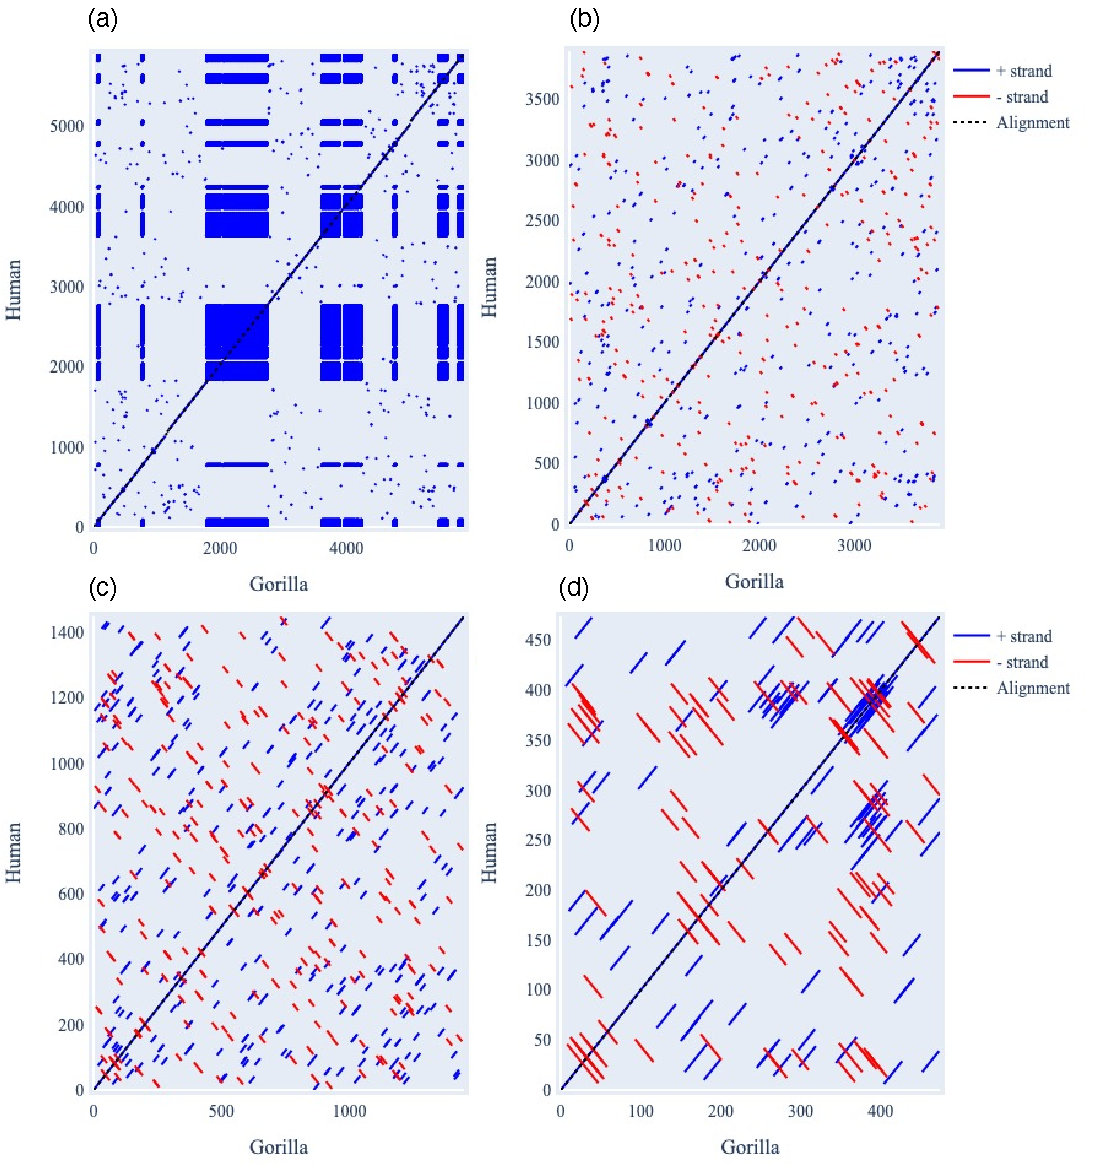
\includegraphics[width=\textwidth]{figures/diagrams/primate_dotplots.pdf}
\caption{Dotplots. Window was 20bp long, a match was considered if $>13$bp of the window of 20 were identical. }
\label{fig:dotplots}
\end{figure}

\section{Models}

In this work I will use two continuous-time models, General Nucleotide (GN), and General Stationary (GS), and one discrete-time model, the Barry and Hartigan (BH) model. 

\subsubsection{GS}

\subsubsection{GNS}


\subsubsection{GTR}


\subsubsection{BH}
GN is a non-stationary nucleotide model for which time-homogeneity between nodes in the tree is the only required constraint \citep{Kaehler2015}. GNS is a stationary nucleotide model, formulated by Von Bing Yap and Gavin Huttley (Personal Communication). The BH model is a general discrete-time Markov process for nucleotides \citep{Barry1987StatisticalEvolution}. The assumptions for each can be found in table \ref{model_assumptions}.
\begin{table}[htbp]
\centering
\begin{tabularx}{0.7\textwidth}{ 
  | >{\centering\arraybackslash}c 
  | >{\centering\arraybackslash}X 
  | >{\centering\arraybackslash}X  
  | >{\centering\arraybackslash}X | }
\hline  
\textbf{Assumption} & \textbf{BH} & \textbf{GN} & \textbf{GS}  \\
\hline 
    Reversibility & - & - & -  \\
    Stationarity & - & - & \checkmark  \\
    Time-Homogeneity  & - & \checkmark & \checkmark \\
    Independent sites & \checkmark & \checkmark & \checkmark\\ 
\hline 
\end{tabularx}
\caption{Markov process assumptions}
\label{model_assumptions}

\end{table}




\subsection{General Nucleotide Markov}

\section{Defining Novel Statistical Measures}

\section{Maximum Likelihood}

For some data, the likelihood of a hypothesis is the probability of the data given that hypothesis. For likelihoods involving substitution models, the tree topology and the values of free parameters are these hypotheses \cite{Lio1998ModelsPhylogeny}. ML methods `fit' a model by returning the model parameters that produce the highest probability of generating the observed sequence data \citep{Edwards1972Likelihood, Felsenstein1981EvolutionaryApproach}. ML is a powerful framework for determining whether there is significant improvement between nested models \cite{Goldman1993StatisticalSubstitution}. One `null' model is considered nested in another if it can be specified simply by imposing restrictions on the parameters of the `alternate' model. For the models of interest, GNS is nested within GN.

A likelihood ratio test (LRT) is a method of comparing nested models \citep{Goldman1993StatisticalSubstitution}. It is a test of whether additional components unique to the alternate model cause a significant improvement in the description of the data \cite{Goldman1993StatisticalSubstitution}. Practically, this involves comparing likelihoods between models, giving a LRT statistic. Suppose the null model is appropriate and the length of the alignment is adequate. In that case, the LRT statistic will be $\chi^2_{df}$ distributed with degrees freedom (df) equal to the difference in the number of free parameter between the models \citep{Lindgren1993StatisticalTheory, Silvey1975StatisticalInference, Kendall1979The2}.

\subsection{Test of Existence}

To achieve this aim I have designed a Likelihood Ratio Test (LRT). The predominant method for examining aspects of sequences' evolution is through the use of \glspl{Substitution model}. \Gls{Maximum Likelihood} methods allow for measuring the support for a hypothesis, (in this case, a \gls{model}), given some data. Whether one hypothesis is better supported than another can be evaluated by using an LRT. Two models fundamental for my LRT are General Nucleotide (GN) and General Nucleotide Stationary (GNS). Their point of difference is that the parameters of a GNS rate matrix must satisfy $\pi\mathbf{Q}=0$, i.e., the process is constrained to be stationary (and thus in equilibrium). Consider an LRT in which GNS is the null and GN is the alternate. If we reject the null, we may conclude that the sequences are more likely to have been generated by a process which is not yet stationary, as this is the only component unique to the alternate.

An LRT as described above is too naive for my objective to test for equilibrium in a single lineage. For a model to be \gls{identifiable} requires an alignment of at least three sequences \cite{Chang1996FullConsistency}. Consequently, a significant result for such an LRT will not reveal which of the taxa is causing the rejection of the null. To test for disequilibrium in a single \gls{edge} requires  modelling a continuous-time process on the edge of interest (herein the foreground edge) and assuming discrete-time processes for the other edges (herein the background edges) \cite{Verbyla2013TheSubstitution}. A discrete-time process is more general (fewer assumptions) than even the GN, making it the ideal background. 

Using mixed discrete- and continuous-time Markov processes, I can test for disequilibrium on a single edge. For such an LRT, the foreground edge assumes GNS for the null, and GN for the alternate. Both hypotheses assume a Barry and Hartigan (BH) model, the most commonly implemented discrete-time process, for the background edges. The modelling of the foreground edge, set apart by the assumption of stationarity, is the only point of difference between hypotheses. For this LRT, a rejection of the null means that the foreground edge was described significantly better with a non-stationary process. Such a result suggests disequilibrium precisely in the foreground edge. Put explicitly, the test will be between the following hypotheses:\\ $\mathbf{H_0}$: the foreground evolved according to the \textbf{GNS}, the background according to BH. \\ $\mathbf{H_1}$: the foreground evolved according to the \textbf{GN}, the background according to BH.\\
\noindent Herein all model fits assume mixed discrete- and continuous-time Markov processes, and a BH process is always assumed for the background edges. For brevity, I will refer to a model by the process assumed on the foreground edge.

\begin{figure}[htbp]
\centering
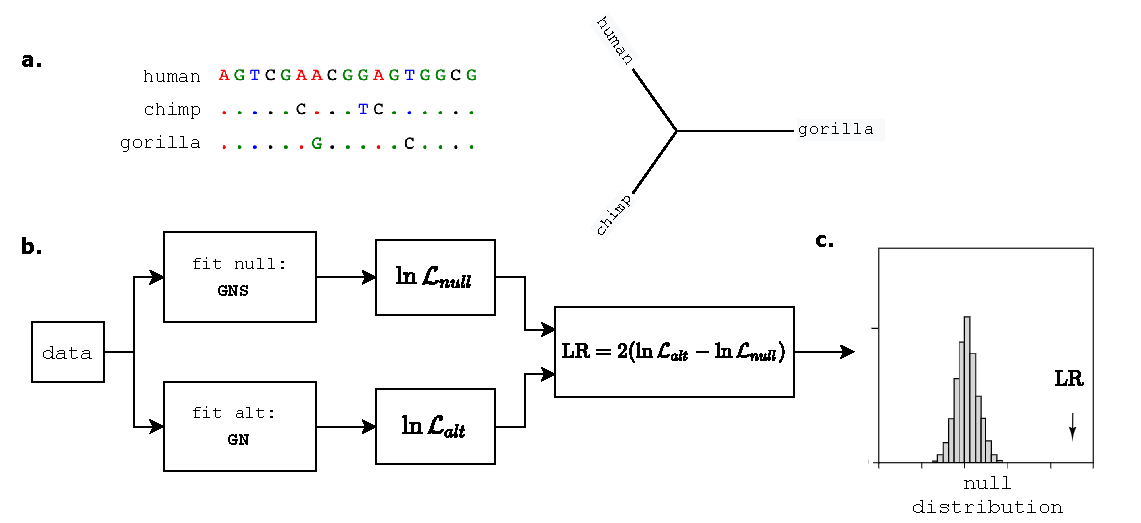
\includegraphics[width=\textwidth]{figures/diagrams/LRT.pdf}
\caption{\textbf{Likelihood Ratio Test.} \textbf{a}, The data: an alignment of orthologous sequences for human, chimp and gorilla, and a phylogenetic tree indicating the relationship between taxa. \textbf{b}, A LRT comparing substitution models, GNS is the null and GN is the alternate. The log-likelihood ($\ln\mathcal{L}$) for each model is obtained via fitting. The likelihood ratio (LR), is the ratio of the $\ln\mathcal{L}$ of the two models. \textbf{c}, the LR statistic is compared to the null distribution. In this case the statistic exceeds the distribution of values we would expect if the null was true, we would thus conclude that process is described significantly better with the alternate (GN) process.}
\label{fig:lrt}
\end{figure}

\subsection{Tests of Equivalence of Process}

For a single alignment of three taxa, a split continuous- and discrete-time model can be specified by the following set of parameters: $( \bm{Q}_{fg}, \bm{P}_{bg1}, \bm{P}_{bg2}, \pi_{0}, b ) $ where $\bm{Q}_{fg}$ is a continuous-time rate matrix describing the foreground edge,  $\bm{P}_{bg1}$ and $\bm{P}_{bg2}$ are discrete-time probability substitution matrices each describing one of the background edges, $\pi_{0}$ is the motif probabilities in the most recent common ancestor, and $b$ is the branch length corresponding to the foreground edge. 

For the adjacent Equivalence of Process test (aEOP) between two alignment $\alpha$ and $\beta$, the null hypothesis constrains both alignments to have the same root motif probabilities and the same rate matrix on the foreground edge, i.e.,  \\
$H_0:$ $\bm{Q}_{fg}(\alpha) = \bm{Q}_{fg}(\beta)$ and $\pi_0(\beta) = \pi_0(\alpha)$. \\
\noindent
The alternate hypothesis allows all parameters to be independent between alignments. 

The temporal Equivalence of Process test (tEOP) is between two edges of the same aligned sequence. In this case, there are two edges of interest, so the process is modelled with all edges as continuous time process. Such a model is specified by the following set of parameters: $( \bm{Q}_{fg1}, \bm{Q}_{fg2}, \bm{Q}_{bg}, \pi_{0}, b_{fg1}, b_{fg2}, b_{bg1}) $, where $\bm{Q}_{fg1}$ and $\bm{Q}_{fg2}$ are continuous-time rate matrices each describing on of the foreground edges,  $\bm{Q}_{bg}$ is a continuous-time rate matrix describing the background edge, $\pi_{0}$ is the motif probabilities in the most recent common ancestor, and $ b_{fg1}, b_{fg2}, b_{fg1}$ is the branch length corresponding to the foreground edge. The null hypothesis constrains both foreground edges to have the same rate matrix, i.e., \\
$H_0:$ $\bm{Q}_{fg1} = \bm{Q}_{fg2}$  \\ 
The alternate hypothesis allows all parameters to be independent. 

\subsection{Bootstrapping Procedure}

\section{Experimental Design}

\subsection{Choosing Seed Alignments}
I require alignments simulated in accordance with a GNS process. One way to obtain data evolving under a GNS process is to exploit the fact that even a non-stationary process will converge to its stationary nucleotide distribution (herein $\pi_{\infty}$) as time goes to infinity. Essentially, I can obtain a GN model from real data, derive its corresponding $\pi_{\infty}$ and use those two things to define a stationary process. The process can be modified to model the background edges as discrete, and I can simulate alignments according to such a specification. This is my chosen simulation method as the resulting alignments are generated from parameters of real data. 

I must consider how the properties of the alignment used for simulation may affect the application of my methods. To address this requires deciding the features of an alignment that may be significant and finding measures that characterise them. I can then choose a selection of alignments that vary systematically by these measures. From each alignment, I can create a data set, resulting in a collection of data sets that differ in a way that reflects the natural variation of real sequence data. Using carefully diversified data allows for a thorough interrogation of my methods and determines how their properties may change when applied to different types of data.

An important measure I require is that of non-stationarity. A direct consequence of a non-stationary process is a change in base composition over time. As follows, an indication of the degree of historical non-stationarity can be obtained from the difference in compositions between sequences in the same alignment. It is worth noting that studies of compositional data often require representation using Aitchison geometry. This representation allows for a consideration of the vulnerability of a composition to the sample it comes from. However, the composition of bases can also be considered as a probability distribution (i.e., $\pi = [\pi_T,\, \pi_G, \, \pi_C, \, \pi_A]$, such that $\pi_i$ where $i= \mathrm{T}, \mathrm{G}, \mathrm{C}, \mathrm{A}$ is the probability of observing the state $i$). In the case of comparing probability distributions, several measures can be used. My selected measure is an information theoretic measure known as Jensen-Shannon Divergence (JSD). JSD measures the similarity between probability distributions. JSD was chosen as it can accommodate multiple distributions, allowing us to apply it to more than two sequences if needed. Additionally, it has an associated true metric, satisfying important mathematical properties (e.g., the triangle inequality). 

A probability distribution also has an associated information content, measured using entropy. Entropy is a fundamental quantity that indicates, in our case, the evenness of base composition. For example, $\pi =[1,\, 0,\, 0,\, 0]$  (a single nucleotide) has zero entropy whilst  $\pi =[0.25,\, 0.25,\, 0.25,\, 0.25]$ (equifrequent nucleotides) has the maximum possible entropy for 4 states. As a measure of compositional diversity, it captures an essential feature of the mode of evolution. For example, an edge that is highly \gls{strand-asymmetric} would have lower entropy than a \gls{strand-symmetric} edge. The base composition may affect the properties of my developed methods. One example being $T_{50}$ for which base composition is used in its computation. Accordingly, the impact of compositions with different entropy is an important feature to consider in the process of method development.

I will approximate the stability of the process using the condition number of the foreground rate matrix. It is important to derive data from numerically stable processes. If a process falls within the scope of being numerically unstable, (meaning computers are poorly equipped to evaluate it using standard settings), I need to be aware of this so I can select a more numerically stable method. An indication of numerical stability is the eigenvector matrix condition number. A matrix condition number is an approximation of the worst case relative change in derivations, for a relative change in the input. For a continuous-time process, the transition rate matrix $\mathrm{Q}$, specifies the instantaneous rates of exchanges between states. $\mathrm{Q}$ is foundational to a given substitution model. The eigendecomposition of $\mathrm{Q}$ is a representation of $\mathrm{Q}$ in terms of its eigenvalues and eigenvectors. Eigendecomposition is fundamental to many methods that I am using and developing (e.g., deriving $\pi_{\infty}$). As an indication of the suitability of a matrix to decomposition, I will use the eigenvector matrix condition number to approximate the numerical stability of a process.

I chose four microbial alignments to generate synthetic data sets and refer to these as seed alignments. As previously stated, I expect that JSD, entropy, and condition number may affect the numerical and or statistical properties of the developed methods. To derive data from numerically stable processes, the seed alignments are chosen from a subset of alignments where the eigenvector condition number is low ($<1.5$). To capture the extent of naturally occurring diversity (measured by JSD) and compositional diversity (measured by entropy), the seed alignments chosen represent the permutations of those extremes. These are: high JSD, low entropy; high JSD, high entropy; low JSD, low entropy; low JSD, high entropy. 

\subsection{Generating Synthetic Alignments that are Stationary, but not Reversible}
I expect the properties of my test to be affected by the number of substitution events that distinguish the sequences in an alignment. The mathematical proof that LRT statistics are $\chi^{2}$ distributed assumes infinite data, that is the alignment is infinitely long. Although it has been shown that a few hundred base pairs can be sufficient for the $\chi^{2}$ to be accurate, this length is ultimately dependent on the number of substitution events \cite{Ota2000AppropriateParameters}. I can increase the number of events in a simulated alignment in two ways, (1) increase the length of the alignment, (2) increase the \gls{branch length} of the tree (increased divergence time). 

It is necessary to determine how my methods are affected by the length of the alignment. I have done this by simulating multiple data sets differing in alignment length for all four seeds. The lengths were chosen to be representative of alignment lengths of my biological application. The shortest sequences I will be using are protein coding genes, for which the average length (using just the 3rd codon position) is about 300bp. For each of the four seeds, I generated data sets of alignment length 300, 3,000, and 30,000.   

It is also necessary to determine the influence of increased branch length. When simulating alignments, I can alter the branch lengths of the generating function. This is a capability that allows me to create synthetic alignments specified by the same process (same $\mathrm{Q}$), but with an increased term of divergence. To address how branch length affects the test, I simulated data sets with an increased branch length for all four seeds. The genetic distance ($d$) (or branch length) is a measure of the expected number of nucleotide substitutions per site. The maximum branch length in my application data sets will be about $d=0.6$. For the long branch simulations, I scaled the tree by a factor of 3. However, branch lengths were capped at $d=0.6$ and the remaining branch lengths were reduced proportionally. 

Each simulation set consisted of 1,000 synthetic alignments. The synthetic alignments are generated from the same function, derived from the parameter estimates from one seed alignment. The simulation process that was performed is described in Figure \ref{fig:simulating_alns}.

\begin{figure}[!ht]
\centering
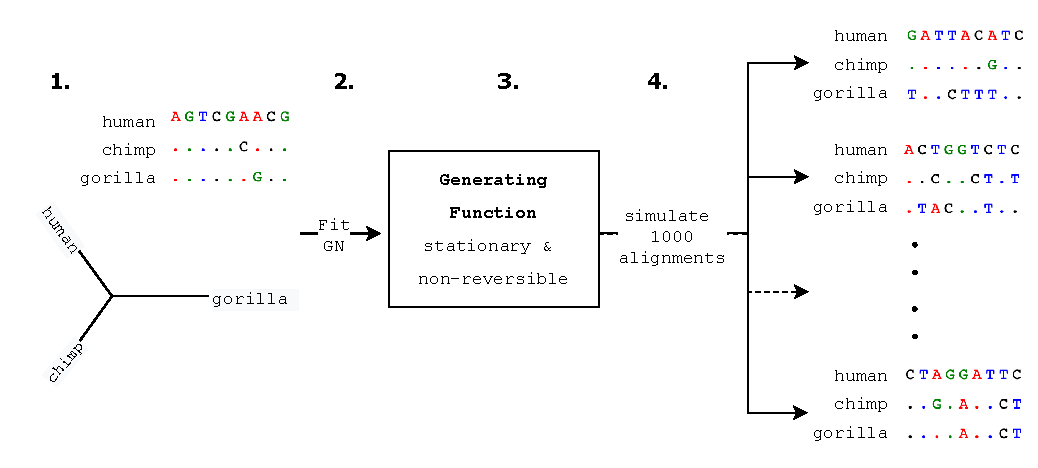
\includegraphics[width=\textwidth]{figures/diagrams/simulating_alns.pdf}
\caption{Creating synthetic data sets whose evolution was stationary but not reversible. \textbf{1,} select seed alignment, \textbf{2}, fit GN mixed model and extract model parameter estimates, \textbf{3}, define generating function using parameter estimates altered to be stationary, \textbf{4}, generate 1000 alignments of length $n$ and branch length scaled by $b$. For all 4 seeds this was performed for n = 300, 3000, 30000, and for each n, b = 1 and 3.}
\label{fig:simulating_alns}
\end{figure}

\section{Algorithmic Implementation}

